\documentclass[10pt,a4paper]{report}

\usepackage[english,italian]{babel}
\usepackage[T1]{fontenc}
\usepackage[utf8]{inputenc}
\usepackage{times}
\usepackage{url}
\usepackage{hyperref}
\usepackage{titlesec}
\usepackage{amssymb,amsmath}
\usepackage{appendix}

\hypersetup{%
    pdfborder = {0 0 0}
}
\usepackage{graphicx}
\usepackage[svgnames]{xcolor} % Required to specify font color
\usepackage{eurosym}


\titleformat{\chapter}[hang] 
{\normalfont\huge\bfseries}{\chaptertitlename\ \thechapter.}{1em}{} 

\titlespacing*{\chapter}{0pt}{5pt}{40pt}

\newcommand*{\plogo}{\fbox{$\mathcal{PL}$}} % Generic publisher logo
\newcommand{\exedout}{%
	\rule{0.8\textwidth}{0.5\textwidth}%
}
\usepackage{listings}
\usepackage{color}
\usepackage{float}
\usepackage{fancyhdr}

\usepackage{ragged2e}
\usepackage{listings}
\usepackage{listingsutf8}
\setlength{\voffset}{-0.5in}
\setlength{\topmargin}{-0.2in}
\setlength{\textheight}{240mm}
\setlength{\textwidth}{142mm}
\setlength{\evensidemargin}{0.3in}
\setlength{\oddsidemargin}{0.3in}

\begin{document}

\begin{titlepage}
\begin{center}
  \bfseries
  \huge UNIVERSITÀ DEGLI STUDI DI PADOVA
  \vskip-.1in
  \rule{\textwidth}{1.5pt}
  \vskip.1in
  \textsc{\LARGE Scuola di Scienze}
  \vskip.2in
  
\includegraphics[scale=.2]{images/logo-unipd}
  \vskip.25in
  \large CORSO DI LAUREA IN INFORMATICA
  \vskip.7in
  \Large PROGETTO \vskip.1in DI
  \vskip.1in
  \LARGE PROGRAMMAZIONE AD OGGETTI
  \vskip.7in
  \emph{\huge PAO: Pets And Owners}
\end{center}

\vskip1in
\hskip.2\textwidth
\begin{minipage}{.75\textwidth}
  \begin{flushleft}
    \bfseries\large \par \emph{Federico Silvio Busetto Matricola:1026925}
  \end{flushleft}
\end{minipage}

\vskip0.9in
\centering
\bfseries
\Large ANNO ACCADEMICO 2015-2016
\end{titlepage}

\pagestyle{empty}
\newpage

\tableofcontents
\newpage
\clearpage

\makeatletter

%----------------------------------------------------------------------------------------
%	CONSTANTS
%----------------------------------------------------------------------------------------

\newcommand{\authorName}{Federico Silvio Busetto}

%----------------------------------------------------------------------------------------
%	HEADER FORMAT
%----------------------------------------------------------------------------------------

\fancyhf{}
\fancyhead[RE]{\small\scshape\nouppercase{\leftmark}}
%\fancyhead[LO]{\small\scshape\nouppercase{\rightmark}}
\fancyhead[LE,RO]{\small\thepage}
%\lhead{\rightmark}
\rhead{\leftmark}

\fancypagestyle{plain}{\fancyfoot[RO,LE]{\thepage}}

\rfoot{\thepage}

\fancyfoot[RO, LE]{\thepage}
\pagestyle{fancy}

\setlength{\parindent}{0pt}

%----------------------------------------------------------------------------------------
%	CODE FORMAT
%----------------------------------------------------------------------------------------

\definecolor{mygreen}{rgb}{0,0.6,0}
\definecolor{mygray}{rgb}{0.5,0.5,0.5}
\definecolor{mymauve}{rgb}{0.58,0,0.82}

\lstset{ 
backgroundcolor=\color{white},
basicstyle=\footnotesize,
breakatwhitespace=true,
breaklines=true,
captionpos=b, 
commentstyle=\color{mygreen},
extendedchars=\true,
inputencoding=utf8/latin1,
frame=single,	 
keepspaces=true,   
keywordstyle=\color{blue}, 
numbers=left,    
numbersep=5pt,
numberstyle=\tiny\color{mygray},
rulecolor=\color{black},
showspaces=false, 
showstringspaces=false, 
showtabs=false,
stepnumber=4,
stringstyle=\color{mymauve},
tabsize=4,
title=\lstname 
}

%----------------------------------------------------------------------------------------
%	CONTENT
%----------------------------------------------------------------------------------------
\chapter{Scopo del Progetto} 
 
\section{Abstract}

E' stata sviluppata un'applicazione Desktop denominata Pets and Owners (da qui in poi PAO). \\
L'applicazione si prefigge di modellare e gestire, molto semplicemente, la parte amministrativa di un piccolo database di una clinica veterinaria fornendo un'interfaccia utente semplice ed intuitiva sviluppata in \textit{Qt}.

\section{Note per la compilazione}
Per compilare il progetto, viene fornito un file .pro. E' necessario utilizzare la versione 5.3.2 o successiva delle librerie \textit{Qt} seguendo le istruzioni riportate all'url a fine pagina \footnotetext[1]{ \url{http://www.studenti.math.unipd.it/index.php?id=corsi\#c688} }
\begin{itemize}
	\item lanciare lo script per la compilazione \textit{qt-532.sh} (non incluso nella consegna)
	\item Posizionarsi nella cartella del progetto contente i sorgenti
	\item lanciare \textit{qmake} 
	\item \textit{lanciare make ./cartellaDiBuild} , cartellaDiBuild conterrà l'eseguibile.\\ Vengono inoltre forniti 3 file \textit{.json} che compongono un piccolo DB dimostrativo da inserire nella stessa cartella contenente il file eseguibile. 
\end{itemize}

L'applicazione è stata sviluppata usando:
\begin{itemize}
	\item QtCreator 3.2.1
	\item Qt 5.3.2
	\item GCC 4.8.6 e GCC 5.3.0
	\item Ubuntu 16.04 Xenial Xerus 64 Bit - Windows 7 Professional 64 Bit, su quest'ultimo aggiungendo le direttive per QMake \textit{ INCLUDEPATH += .\ e  DEPENDPATH += .\ } 
\end{itemize}

\textbf{Nota:} Su Windows la build viene eseguita correttamente da QtCreator ma usando MinGW da linea di comando si potrebbe incappare in un'errore, si sconsiglia quindi una compilazione sotto questo ambiente. Ulteriori dettagli seguendo il secondo link indicato a fine pagina. \footnotetext[2]{ \url{http://goo.gl/NQGlk3} }

\section{Vincoli obbligatori}
\begin{itemize}
\item \textbf{Definizione ed utilizzo di una gerarchia G di tipi di altezza $\geq 1$ e larghezza $\geq 1$}: \\ A tal proposito è stata sviluppata una gerarchia di Visite, descritta in seguito.
\item \textbf{ Definizione di un opportuno contenitore C, con relativi iteratori, che permetta inserimenti, rimozioni, modifiche.}: E' stato sviluppata una classe \textit{PAOContainer} per la gestione delle visite che verrà illustrata nella sezione \textit{Orientamento agli oggetti}
\item \textbf{Utilizzo del contenitore C per memorizzare oggetti polimorfi della gerarchia G.} \\Il \textit{PAOContainer} memorizza e gestisce puntatori polimorfi di \textit{AbstractVisit}, l'uso di puntatori è necessario per utilizzare polimorfismo e i metodi virtuali descritti in seguito.
\item \textbf{Il front-end dell’applicazione è una GUI sviluppata usando il framework Qt.}
\end{itemize}
\ % Scopo del progetto: include correttezza, note su compilazione, Vincoli obbligatori,scopi
\chapter{Orientamento agli Oggetti} 
 
\section{Descrizione delle Gerarchie}

L'intera applicazione si compone di 20 classi (12 per le gerarchie principali, 3 di tipi utilità e 6 per la GUI).
La gerarchia principale, nonché la più importante è la gerarchia delle visite. Essa si compone di quattro classi:
\begin{itemize}
	\item \textit{\textbf{AbstractVisit}}: Una classe virtuale pura (non istanziabile direttamente), contiene 3 metodi virtuali puri, uno per scrivere su file i campi contenuti nelle classi derivate, uno per calcolare il prezzo finale della visita e uno di utilità che ritorna una stringa indicante il tipo di Visita.
	\item \textit{\textbf{BasicVisit}}: Deriva pubblicamente da \textit{AbstractVisit} e calcola il costo finale, \textit{override} dell'apposito metodo virtuale puro, restituendo il prezzo base.
	\item \textit{\textbf{VaccineVisit}} Deriva pubblicamente da \textit{AbstractVisit} e calcola il costo finale tramite override,  come il doppio del prezzo base di una visita di base.
	\item \textit{\textbf{SpecializedVisit}} Deriva pubblicamente da \textit{AbstractVisit} e calcola il costo finale con un 30 \% aggiuntivo rispetto al prezzo di un Vaccino.
\end{itemize} 

\subsection{Utilità e ruolo dei tipi}
 Oltre alle quattro classi descritte sopra, ve ne sono altre:
 \begin{itemize}
 	\item \textit{\textbf{AbstractOwner}}: Modella un generico proprietario di animali (può essere un veterinario), è una classe virtuale pura, madre della seconda gerarchia. Contiene due metodi virtuali puri, usati per restituire una stringa e per salvare i dati su file; contiene inoltre un puntatore ad una classe \textit{OwnerAccount} e una stringa per memorizzare il Codice Fiscale.
 	\item \textit{\textbf{Owner}}: Deriva pubblicamente da \textit{AbstractOwner} e rappresenta un proprietario privato di animali. Contiene un puntatore ad una classe \textit{OwnerData}.
 	\item \textit{\textbf{OwnerAccount}}: Utilizzata per funzionalità future. Permette di distinguere se un utente è o no un veterinario. Inoltre fornisce delle funzionalità di Encryption della password, memorizzata tramite un hash.
 	\item \textit{\textbf{OwnerData}}: Contiene le informazioni di un proprietario, quali nome, cognome e informazioni di contatto, queste ultime tramite un campo dati di tipo \textit{ContactInfo}
 	\item \textit{\textbf{ContactInfo}}: Utilizzata in \textit{OwnerData}, descrive indirizzo fisico, mail e numero di telefono di un proprietario.
 	\item \textit{\textbf{Animal}}: Descrive un animale generico. E' una classe virtuale pura, madre della terza gerarchia utilizzata dall'applicazione.
 	Contiene due metodi virtuali puri per restituire una stringa e per salvare i campi dati su file. Contiene inoltre un campo ad una classe \textit{AnimalData}
 	\item \textit{\textbf{Pet}}: Estende pubblicamente \textit{Animal} e rappresenta un animale domestico, caratterizzato dal tipo (Cane, Gatto, Volatile o Altro), dal colore del pelo e dalla razza dell'animale.
 	\item \textit{\textbf{AnimalData}}:Contiene le informazioni essenziali di un animale, quali nome, data di nascita, sesso e peso ed eventualmente data di applicazione del microchip.
 \end{itemize}
 
 Vi sono poi due classi d'utilità: Il contenitore delle visite e il database vero e proprio. Le ulteriori sei classi che modellano la parte grafica verranno trattate nella sezione \textit{Interfaccia Grafica}.
 
 \begin{itemize}
 	\item \textit{\textbf{PaoDB}}: Gestisce gli utenti tramite una \textit{QMap<QString, AbstractOwner*>}, gli animali tramite una \textit{QMap<QString, Animal*>} e le visite tramite il contenitore preposto, \textit{PaoContainer}. \\ La classe fornisce metodi per inserire, modificare, rimuovere proprietari, animali e visite, per leggere i dati delle tre entità da file e caricarli in memoria e per salvarli su disco rigido in formato \textit{JSON}
 \end{itemize}
 
 
 \subsection{Descrizione del contenitore}
 La classe PaoContainer altro non è che una lista che permette inserimenti in testa ed in coda. \\Essa si avvale di due classi interne private: \textit{node}, la lista vera e propria di nodi e \textit{SmartPointer} per la gestione della memoria condivisa, così come visto durante il corso. 
 \\ Il contenitore mette a disposizione per iterare sui suoi elementi due tipi di iteratori: Un \textit{iterator} per accedere normalmente agli elementi del contenitore e un \textit{const\_iterator} utilizzato per la sola lettura. La classe \textit{PaoContainer} è amica degli iteratori e viceversa, questo permette agli iteratori di accedere alla parte privata di \textit{PaoContainer} e a \textit{PaoContainer} di accedere alla parte privata degli iteratori. \\ 
 
 \textit{PaoContainer} fornisce funzioni per determinare la sua dimensione (\textit{size()}), per verificare se è vuoto (\textit{isEmpty()}) per l'inserimento in testa (\textit{push\_front}) e in coda (\textit{push\_back}), per ottenere una visita da modificare, per ritornare l'iteratore iniziale e l'iteratore \textit{Past the End} e per rimuovere visite.
 I suoi due campi dati sono uno \textit{SmartPointer} che punta alla testa del Contenitore e un intero che ne rappresenta la size, cioè il numero di elementi contenuti. Container fornisce inoltre l'\textit{overloading} dell'operatore di accesso a membro \textit{operator[]}, altri operatori sono stati ridefiniti nelle classi interne.
 
\section{Incapsulamento}

Si è scelto di garantire un incapsulamento fornendo alle varie classi, alcune funzioni cercando di usare, quanto più, metodi costanti e  gli specificatori di accesso \textit{private} e \textit{protected} rendendo \textit{public} solo dei metodi \textit{getter} e \textit{setter} di interfaccia.
\\Questo, da una parte permette di non accedere direttamente ai campi dati ma dall'altra espone in parte la struttura delle classi.
Alla fine, dopo averci riflettuto su a lungo, per quanto la soluzione non sia delle migliori e visti gli scopi del progetto è risultata essere la scelta più conveniente. \footnotetext[3]{ \url{http://goo.gl/CPF3up} } \footnotetext[4]{ \url{https://dzone.com/articles/getter-setter-use-or-not-use-0} }

Un incapsulamento soddisfacente è stato ottenuto per il salvataggio dei dati delle singole classi su file, dove ogni classe è responsabile di salvare i propri campi dati.

\section{Modularità}

Ogni classe è stata suddivisa in un file di header .h contenente le dichiarazioni e in un file .cpp contenente le definizioni implementative. Si è cercato inoltre di suddividere i compiti in varie funzioni secondo il principio della \textit{Single-Responsibility}, ovvero un compito specifico per ciascuna funzione.

\section{Estensibilità $\backslash$ Evolvibilità}

Si è scelto di far partire le tre gerarchie con delle classi astratte, in modo da permettere una eventuale estensione futura del software. 
Ad esempio, si potranno creare dei diversi tipi di proprietario derivando da \textit{AbstractOwner}, per rappresentare uno zoo o un parco nazionale. 
Si potrà derivare \textit{Animal} per nuove categorie di animali (esotici, selvaggi, da giardino) e soprattutto si potranno creare nuovi tipi di visite a partire da \textit{AbstractVisit}, includendo, ad esempio, un accertamento radiologico con un prezzo appositamente calcolato.
\\ 

\subsection{Esempi d'uso di codice polimorfo}
\lstinputlisting[language=C++, firstline=6, lastline=9]{cpp/specializedvisit.cpp} 
Un esempio di \textit{override} di un metodo virtuale puro, per il calcolo del costo finale di una visita specialistica.\\

\lstinputlisting[language=C++, firstline=120, lastline=135]{cpp/vetcontrol.cpp} 

Un esempio di RTTI per estrarre i dati dei proprietari da aggiungere alla tabella.\\

\lstinputlisting[language=C++, firstline=14, lastline=18]{cpp/specializedvisit.cpp} 

Sempre sulla visita specialistica, un esempio di \textit{override} per salvare i dati su file.\\

\textit{\textbf{Nota:}} Si voleva utilizzare il marcatore esplicito \textit{override} previsto da \textit{C++11}, in modo da rendere più chiaro quali metodi sono degli override all'interno delle classi, tuttavia ciò non è stato possibile in quanto la versione di GCC presente in laboratorio non supportava ancora tale funzione.

\section{Efficienza $\backslash$ Robustezza}
Si è cercato di rendere robusta soprattutto l'interfaccia grafica tramite dei controlli elementari sui campi dati inseriti, ad esempio le chiavi non possono essere una \textit{QString} vuota. % Descrizione di G, ruolo dei tipi di G, incapsulamento, modularita (Logica, grafica, GUI),estensibilità/evolvibilità polimorfismo, efficienza, robustezza
\chapter{Funzionalità} 

Le funzionalità messe a disposizione dall'applicazione \textit{PAO} sono:

\begin{itemize}
	\item \textit{\textbf{Aggiunta $\backslash$ Rimozione $\backslash$ Modifica}}: Di proprietari e animali sfruttando le peculiarità di \textit{QMap}. Ogni modifica avverrà tramite un inserimento di nuovi valori utilizzando la stessa chiave. Dal punto di vista grafico però non è il massimo.
	\item \textit{\textbf{PaoContainer}}: Il contenitore, già descritto in precedenza. Permette la modifica, l'aggiunta e la rimozione di Visite.
	\item \textit{\textbf{Encryption}}: Ogni classe \textit{AbstractOwner} ha un campo di tipo \textit{OwnerAccount} che a sua volta memorizza un \textit{QCryptographicHash} che rappresenta l'hash della password di un utente. La classe è pronta all'uso, in vista di future evoluzioni del software che potranno includere una schermata di login e un lato client.
	\item \textit{\textbf{Salvataggio su file}}: Tramite apposite funzioni, viene aperto un file in sola scrittura per ogni tipo di entità principale (Owner, Animal e Visit), viene allocato un \textit{QJsonObject} principale e successivamente, viene creato un \textit{QJsonArray} di \textit{QJsonObject}. \\ Per ogni elemento dei contenitori, vengono invocati i metodi \textit{save} dei singoli oggetti definiti nelle varie classi. Il contenuto viene quindi riversato nell'array ed infine, tramite il metodo \textit{write} di \textit{QJsonDocument}, viene effettuata la scrittura vera e propria su file.  
	\item \textit{\textbf{Caricamento da file}}: Viene fatto il processo opposto a quello di salvataggio, leggendo dai file scritti in precedenza tramite l'invocazione di apposite funzioni e i costruttori \textit{JSON} dei vari oggetti. Per implementare il tutto si è fatto uso della documentazione \textit{Qt} online. Un esempio di documentazione utilizzata è reperibile a fondo pagina \footnotetext[5]{ \url{https://doc.qt.io/qt-5/qtcore-json-savegame-example.html}}.
\end{itemize} 

\section{Interfaccia Grafica (GUI)}

Per la parte di interfaccia grafica si è cercato di dividere quanto più possibile la parte logica che interagisce con il database (il model) dalla parte grafica vera e propria (la view), secondo un pattern \textit{MVC}.\\ Per implementare questo pattern si è preferito creare due classi principali, descritte di seguito, piuttosto che avvalersi del MVC stile \textit{Qt} anche se quest'ultimo avrebbe garantito maggior riusabilità del codice e risultati migliori. 
Le due classi sviluppate sono:

\begin{itemize}
	\item \textit{\textbf{vetcontrol}}: Interagisce col database, predisponendo gli elementi nella tabella e richiamando i metodi di inserimento, modifica e rimozione di elementi. Apre inoltre i pannelli per l'inserimento e la modifica di nuovi elementi. \\Si è pensato di generare i nuovi pannelli all'interno del controller, anche se sarebbe stata una cosa prettamente di competenza della view, in quanto questi ultimi interagiscono anche loro col database sottostante. 
	\item \textit{\textbf{vetview}}: La vista amministrativa principale. Questa vista è divisa in tre sezioni tramite cinque \textit{QGroupBox}. \\A sinistra abbiamo i pulsanti per aprire i pannelli di inserimento, a destra, dinamicamente, viene visualizzato uno dei tre \textit{QGroupBox} per modifica e rimozione (in base al valore della \textit{QComboBox} presente nel \textit{Widget} centrale)  e al centro abbiamo, oltre alla già menzionata \textit{QComboBox}, un \textit{QTableWidget} e un \textit{QPushButton} d'uscita. \\Una funzione principale prepara la GUI, impostando i vari elementi grafici e un'altra imposta le \textit{connect} per associare tra loro vari eventi secondo il sistema di \textit{signal} e \textit{slot} fornito dal framework \textit{Qt}. \\La maggior parte dei metodi di questa classe, sono metodi privati, non accessibili all'esterno della stessa. 
\end{itemize}

Rimangono quattro classi che implementano i pannelli di inserimento e quello di modifica.
\begin{itemize}
	\item \textit{\textbf{AddOwnerDialog}}: Permette l'inserimento di proprietari. Delle \textit{QLineEdit} permettono all'utente di inserire i vari dati, uno slot pubblico si occuperà al momento del salvataggio di fare un minimo di controlli, creare un \textit{Owner} e aggiungerlo alla mappa del database passando attraverso il controller.
	\item \textit{\textbf{AddAnimalDialog}}: Analoga a \textit{AddOwnerDialog}
	\item \textit{\textbf{AddVisitDialog}}: Analoga a \textit{AddOwnerDialog} e a \textit{AddAnimalDialog}
	\item \textit{\textbf{EditVisitDialog}}:Permette la modifica di una visita selezionata. E' lo stesso pannello di inserimento, riadattato per disabilitare alcune componenti grafiche.
\end{itemize}

\begin{figure}[H]
	\centering
	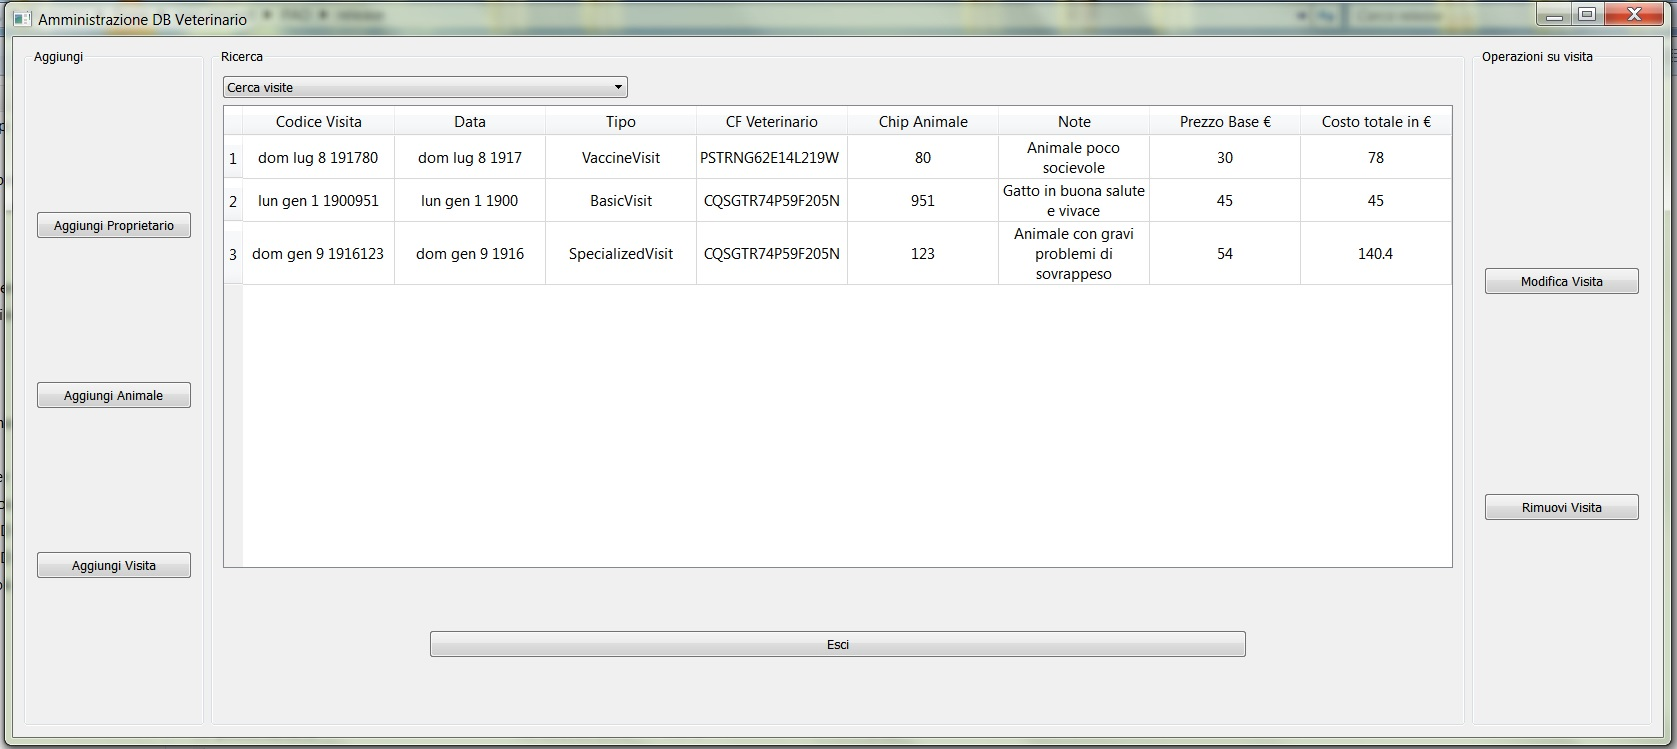
\includegraphics[width=\textwidth]{images/main_view_visits.jpg}
	\caption{La finestra d'amministrazione principale con le visite caricate}
\end{figure}


\begin{figure}
	\centering
	\begin{minipage}{0.45\textwidth}
		\centering
		%\exedout % first figure itself
		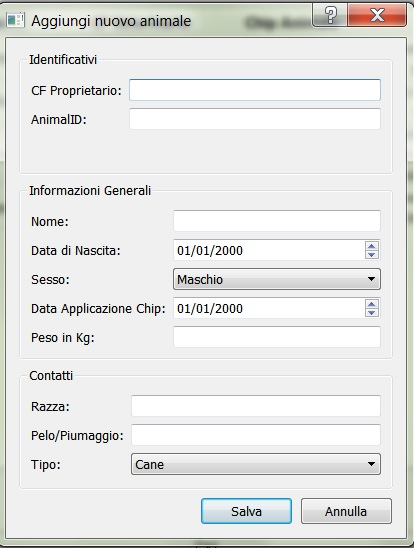
\includegraphics[width=.5\linewidth]{images/addAnimal_view.jpg}
		\caption{Pannello Aggiunta animali}
	\end{minipage}\hfill
	\begin{minipage}{0.45\textwidth}
		\centering
		%\exedout % first figure itself
		\includegraphics[width=.5\linewidth]{images/editvisit_view.jpg}
		\caption{Pannello Modifica Visite}
	\end{minipage}
\end{figure}

\subsection{Nota}
All'inizio la vista è impostata su modalità \textit{Owner} ma la tabella appare vuota. Cambiando il valore della \textit{QComBobox} verranno caricati dinamicamente i dati richiesti.

 % quante, quali, qualità e GUI
%\include{final_thoughts}

%\appendix

%\input{glossario}
\end{document}